\newcommand{\nuT}{\nu_T}
\newcommand{\nut}{{\widetilde \nu}}
\newcommand{\Dop}{{\cal D}}
\newcommand{\Dopu}{{\cal D}_u}
\newcommand{\Dopv}{{\cal D}_v}
\newcommand{\Dopw}{{\cal D}_w}

% -------------------------------------------------------------------------------------------------------------
\section{Turbulence models}

The typical RANS model for the incompressible Navier-Stokes equations which uses the
Boussinesq eddy viscosity approximation is
\begin{align*}
  \partial_t u_i + u_k \partial_{x_k} u_i + \partial_{x_i} p &= 
             \partial_{x_k}\Big( (\nu+\nuT) (\partial_{x_k} u_i + \partial_{x_i} u_k) \Big) \\
   \tau_{i,j} &= (\nu+\nuT) (\partial_{x_k} u_i + \partial_{x_i} u_k) \\
    \nut &= \nu + \nuT
\end{align*}
where $\nuT$ is the turbulent eddy viscosity.

\subsection{Wall Shear Stress} \label{sec:wallShearStress}
The stress on a wall with normal $\nv$ is 
\begin{align*}
   \tauv_{\rm wall} &= \tauv \cdot \nv 
\end{align*}
The shear stress is the tangential component of this wall stress,
\begin{align*}
   \tauv_{\rm shear} &=  \tauv_{\rm wall} - (\nv\cdot\tauv_{\rm wall})\nv \\
                     &= \tau_{i,j}n_j - (n_k\tau_{k,j}n_j )n_i 
\end{align*}

In two-dimensions for a horizontal wall, $\nv=[0,1]^T$ and the wall shear stress is 
\begin{align*}
   \tau_w = (\nu+\nuT) (\partial u / \partial y + \partial v / \partial x )
\end{align*}
Question : Is $\nuT$ on the wall equal to zero always?

In three-dimensions we define scalar wall shear stress $\tau_w$ in terms of the
tangential component of the velocity at the wall, $\uv_t$, 
\begin{align*}
   \tau_w &= \tv \cdot \tauv \cdot \nv,  \\
   \uv_{\rm tan} &= \uv - (\nv\cdot\uv)\nv , \\
   \tv &= \uv_{\rm tan} / \vert \uv_{\rm tan} \vert . 
\end{align*}


Given the definition $\tau_w$ we can define (see for example Wilcox~\cite{Wilcox})
\begin{align*}
     u_\tau = \sqrt{ \tau_w \over \rho }  &\qquad  \mbox{Friction velocity} \\
     \uv^+ = \uv/u_\tau    & \qquad \mbox{non-dimensional velocity for near wall region} \\
     y^+ = u_\tau y/\nu  & \qquad \mbox{non-dimensional length for near wall region} \\
      U = \vert \uv_{\rm tan} \vert  & \\
  {U\over u_\tau} = {1\over\kappa} \ln {u_\tau y\over\nu} ~+C &\qquad 
             \mbox{law of the wall, $\kappa$=K\'arm\'an's constant} \\
   U^+ = {U\over u_\tau} &\qquad \mbox{non-dimensional velocity for near wall region} \\
   U^+ = {1\over\kappa} \ln( E y^+)  & \qquad \mbox{law of the wall, $E$=surface roughness parameter} \\
%  U = U_e - u_\tau g( y/\Delta) & \qquad \mbox{Clauser defect law} \\
%   k_s^+ = {u_\tau k_s \over \nu} &\qquad \mbox{normalized surface roughness}
\end{align*}

For a horizontal wall, with flow in the x-direction, and $\rho=1$, and assuming $\nuT(0)=0$, 
we have
\begin{align*}
  u_\tau &= \sqrt{ \nu  U_y(0)} \\
  y^+ &= y \sqrt{ U_y(0)/\nu } \\
  U(y) &= {\sqrt{ \nu U_y(0)} \over\kappa} \ln\left[ E y \sqrt{U_y(0)/\nu} \right]
\end{align*}


% ------------------------------------
\subsection{Wall Functions}\label{sec:WallFunctions}
\newcommand{\uTau}{u_\tau} % friction velocity
\newcommand{\OmegaWallLaw}{\Omega_{\rm wall-law}}

Wall functions are used to apply approximate boundary conditions in numerical simulations.
They are used when the grid does not resolve the boundary layer. 

% Figure~\ref{fig:lawOfTheWallFunction} shows a plot of $U$ verses $\uTau$ for the law-of-the wall function
\begin{figure}
\begin{center}
  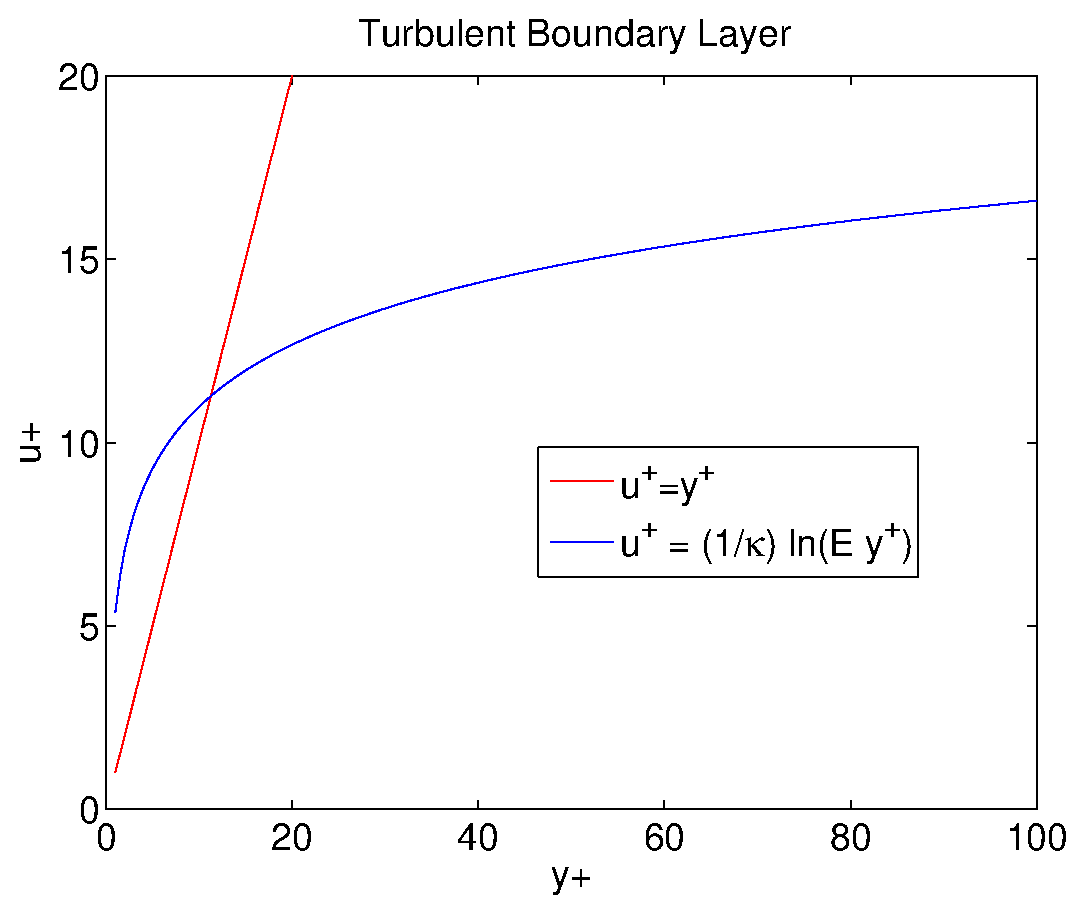
\includegraphics[width=8.cm]{\cgDoc/ins/turbulenceModels/turbulentBoundaryLayerNoLog}
  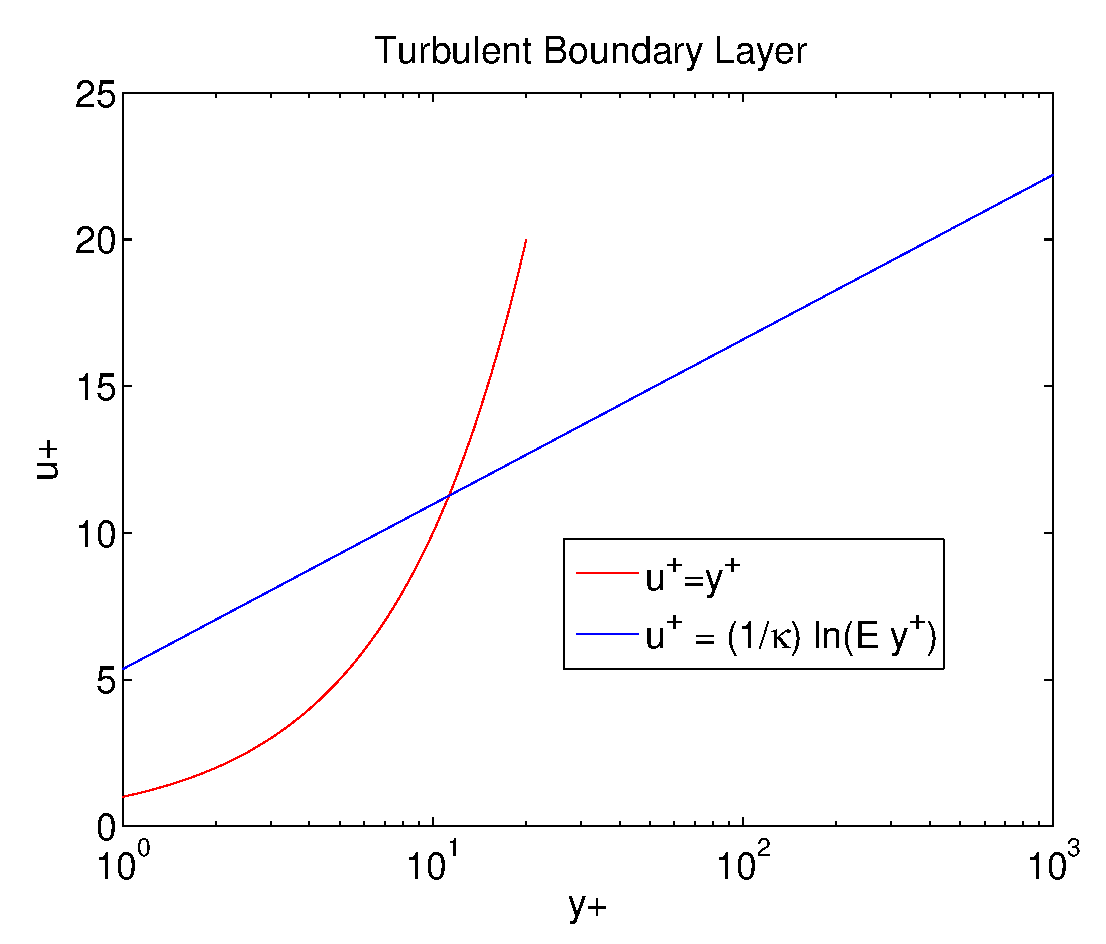
\includegraphics[width=8.cm]{\cgDoc/ins/turbulenceModels/turbulentBoundaryLayer}
\end{center}
\caption{A turbulent boundary layer is thought to have an inner viscous sublayer where $u^+=y+$
  and an outer log-layer where $u^+ = \kappa^{-1}\ln(E y^+)$.}
\label{fig:turbulentBoundaryLayer}
\end{figure}


The basic wall function approach assumes that the first grid point off the
wall is located in the region where the law of the wall is valid.
If $y_p$ denotes the first grid point next to the wall then the law of the
wall relates the tangential component of the velocity in the direction of the flow, $U(y_p)$,
to the wall shear stress, 
\begin{align}
  U(x,y_p) &= {\uTau \over\kappa} \ln\left[ E y_p \uTau/\nu \right] \label{eq:lawOfWall2} \\
    U^+    & = \kappa^{-1} \ln(E y^+) \\ 
       \uTau & = \sqrt{ \nu u_y(x,0)} = \sqrt{\tau_w/\rho} \quad\mbox{(friction velocity)}
\end{align}
Here $E=9$ for smooth walls and $\kappa=0.41$. 
The law of the wall is thought to be valid in an attached turbulent boundary layer 
in region $\OmegaWallLaw = \{ ~\xv~ \vert 20 \le y^+ \le 100\}$. 
This condition replaces the wall no-slip boundary condition, $U(0)=0$,   on the component of the velocity
in the direction of the flow (i.e. $U = \tv\cdot\Uv$ where $\tv=\Uv/\vert \Uv \vert$) . 
The condition is combined with the BC $\nv\cdot\Uv(0)=0$. In 3D we also need a condition on
the other tangential component, which I think that we set to zero.

Note that $\lim_{y\rightarrow 0} U_y(x,y) \ne u_y(x,0)$ since the law of the wall does not hold for $y^+ < 20$.
Thus the wall shear stress is defined using the fully resolved solution $u(x,y)$ and not the Reynold's averaged solution $U(x,y)$.

\bogus{
We also know that the momentum equations are satisfied at the point $p$: 
\begin{align*}
    \uv(p)\cdot\grad\uv + \grad p = \grad\cdot( \tauv )
\end{align*}

We have something like
\begin{align*}
    U U_x + v U_y + p_x = \partial_x( 2\nut U_x + \nut v_y) + \partial_y( \nut v_x + \nut U_y)
\end{align*}
which discretized becomes something like
\begin{align*}
    U D_{0x} U + v D_{0y} U + p_x = \partial_x( 2\nut U_x + \nut v_y) + \partial_y( \nut v_x )
                                +  \Big((\nut U_y)(p+1)- (\nut U_y)(0))\Big)/(2 {\Delta y})
\end{align*}
We then supposedly use~\eqref{eq:lawOfWall2} to replace $U_y(0)$ in this last equation in terms
of $U(p)$. 


}


In the literature it is usually stated that the law of the wall is used to give $\tau_w$, given a value $U(x,y_p)$, and
this $\tau_w$ is used in the momentum equations to evaluate $\grad\cdot(\tauv)$ at the point $y_p$. This doesn't
seem correct. The correct way would be to use the law of the way to evaluate $U_y(x,y)$ for a point near the
wall and use this value in the momentum equation.

By differentiating the law of the wall w.r.t to $y$ we get
\begin{align}
  U_y(x,y) &= {\uTau \over\kappa y} ~,~
  U_{yy}(x,y) = - {\uTau \over\kappa y^2}, 
\end{align}
which are valid for $\xv\in\OmegaWallLaw$. 
% Subsituting these expressions into the momentum equations , we can replace all occurences of $U(x,y$
% by $U_y(x,0)$. Thus we have an equation for $U_y(x,0)$ and use~\eqref{eq:lawOfWall2} to give $U(x,y_p)$.  


So maybe we can implement the wall function by solving the full momentum equations on the first line in and
by defining $U(x,0)$ from the two equations
\begin{align}
  { U(x,y_p)-U(x,0) \over \Delta y } &\approx U_y(x,y_p/2) \approx {\uTau \over\kappa} {1\over y_p/2 } \\
  U(x,y_p) &= {\uTau \over\kappa} \ln\left[ E y_p \uTau/\nu \right]
\end{align}
The second equation gives $\uTau$ as an implicit function of $U(x,y_p)$, $\uTau=F(U(x,y_p))$
\begin{align} 
  U(x,y_p)  & = {\uTau \over\kappa} \ln( E y_p \uTau/\nu )   \leftrightarrow \uTau = F(U(x,y_p)) \label{eq:low} \\
\end{align}
These equations can be thus used to eliminate $\uTau$ to give $U(x,0)$ in terms of $U(x,y_p)$, giving
\begin{align}
  U(x,0) & = U(x,y_p) -  {\uTau \over\kappa} { \Delta y \over y_p/2 } \\
         & = U(x,y_p) -  {2\over \kappa} F(U(x,y_p))
\end{align}
We can approximate this non-linear boundary condition by linearizing about some current guess for $U(x,y_p)\approx U_p^0$. 
Suppose that $F(U_p^0)=\uTau^0$. Then expanding $F(U_p^0 + \delta U)$ gives 
\begin{align*}
  F(U_p^0 + \delta U) &\approx F(U_p^0) + {\partial F \over \partial U}(U_p^0) \delta U 
\end{align*}
Differentiating the expression~\eqref{eq:low} with respect to $U$ gives (*check this*)
\begin{align*}
  {\partial F \over \partial U} &=  
           {\partial \uTau \over \partial U} = { \kappa \over 1+ \ln( E y_p \uTau/\nu) }  = {  \kappa \over 1 + \kappa U /\uTau } 
\end{align*}
Whence the linearized boundary condition is 
\begin{align*}
  U(x,0) & = U(x,y_p) -  2\kappa^{-1}F(U(x,y_p)) \\
         & = U(x,y_p) -  2\kappa^{-1}\Big( F(U_p^0) + F_U(U_p^0)( U(x,y_p) -U_p^0 ) \Big) \\
         & = \Big(1 - 2\kappa^{-1} F_U(U_p^0)\Big) U(x,y_p) - 2\kappa^{-1}\Big( F(U_p^0) - F_U(U_p^0)~U_p^0 \Big) \\
         & = A_w U(x,y_p) + B_w \\
  A_w(U_p^0) & = 1 - {2\over 1 + \kappa U_p^0 /\uTau^0 } = {\kappa U_p^0 /\uTau^0 - 1 \over \kappa U_p^0 /\uTau^0 +1}
             = {\ln(E y_p^+) -1 \over \ln(E y_p^+) + 1} \\
  B_w (U_p^0) & = - 2\kappa^{-1} \uTau^0 + {2 \over 1 + \kappa U_p^0 /\uTau^0 }~U_p^0 
              = { - 2\kappa^{-1} \uTau^0 \over \kappa U_p^0 /\uTau^0 +1}
%   F_U(U_p^0) &= {  \kappa \over 1 + \kappa U_p^0 /\uTau^0 } =  {\kappa \over 1 + \ln( E y_p \uTau^0/\nu) }
\end{align*}
This gives a boundary condition involving $U(x,0)$ and $U(x,y_p)$ linearized about a state $(U_p^0,\uTau^0)$ that
satisfies the law of the wall. Also note that $0< A_w <1 $ if $E y_p^+ > e$ (recall that $E=9$ for smooth walls).

From Wilcox~\cite{Wilcox}, the boundary conditions for $k$ and $\epsilon$ for the $k-\epsilon$
model are then given by
\begin{align*}
  k = { \uTau^2 \over \sqrt{C_\mu}} , \qquad \epsilon = {\uTau^3 \over \kappa y}
\end{align*}
These could be imposed on the first line in, $y=y_p$ ? 


{\bf Solving for $\uTau$ from the law of the wall:} Given a value $U_p=U(x,y_p)$ we need to be able to
solve the nonlinear equation~\eqref{eq:low}
to compute a value for $z=\uTau$ satisfying 
\begin{align*}
     G(z) &\equiv \kappa^{-1} z \ln( A z) - U_p = 0  \\
     A &= E y_p/\nu \\
     G'(z) &= \kappa^{-1} ( 1 + \ln( A z) )
\end{align*}
Note: If $U_p=0$ then $z=1/A$. 
Using Newton's method we get the iteration,
\begin{align*}
     z^{k+1} &= z^k - { G(z^k) \over G'(z^k)}
\end{align*}
There could be trouble with this iteration if $G'(z^k) = 0$, that is when $A z^k = e^{-1}$. 
However, if $U_p\ge 0$ then $Az$ should satisfy $ Az \ge 1 > e^{-1}$. This can seen from the fact that
$z\ln(Az) \le 0 $ for $Az \le 1$. Therefore $G(z)=0$ at $z=1/A$ and thus $z$ should always satisfy $z>1/A$ which
imples $G'(z) \ge \kappa^{-1}$.

An initial guess for $z$ may come from the expression
\begin{align*}
     z &= {\kappa U_p \over \ln(E y_p^+)}, \quad \rightarrow \quad 
            {\kappa U_p \over \ln(100 E )} < z^0 < {\kappa U_p \over \ln(20 E)}
\end{align*}
if we assume that $y_p^+ \in [20,100]$. 


In a boundary layer we might expect that as $R_e \rightarrow \infty$,
\begin{align*}
     \tau_w &\sim R_e^{-1/2} \ll 1  \\
     \uTau  &\sim R_e^{-1/4} \ll 1  \\
\end{align*}
The viscous length scale is $\lambda_{\rm min}=\nu/\uTau$. 
If the first grid line is at $ y_p = M \lambda_{\rm min}$  (i.e. at $y^+ = M$) with $M \in [20,100]$, then
\begin{align*}
     A & = E y_p/\nu  = E M/\uTau \sim E M  R_e^{1/2} \gg 1 \\
     A\uTau &=  E M 
\end{align*}
The product $E M \approx 9 M $ is quite large.  

Figure~\ref{fig:lawOfTheWallFunction} shows a plot of $U_p$ verses $\uTau$ for the law-of-the wall function
We see that a linear fit $\uTau = a U_p + 1/A$ is a good approximation where the constant
$a$ is chosen as 
\[
   a = { \uTau^m - 1/A \over \kappa^{-1}\uTau^m \ln(A \uTau^m)}
\]
so that $U_p = \kappa^{-1}\uTau^m \ln(A \uTau^m)$ for some $\uTau^m$ which represents some
average value for the expected values for $\uTau$. 
\begin{figure}
\begin{center}
  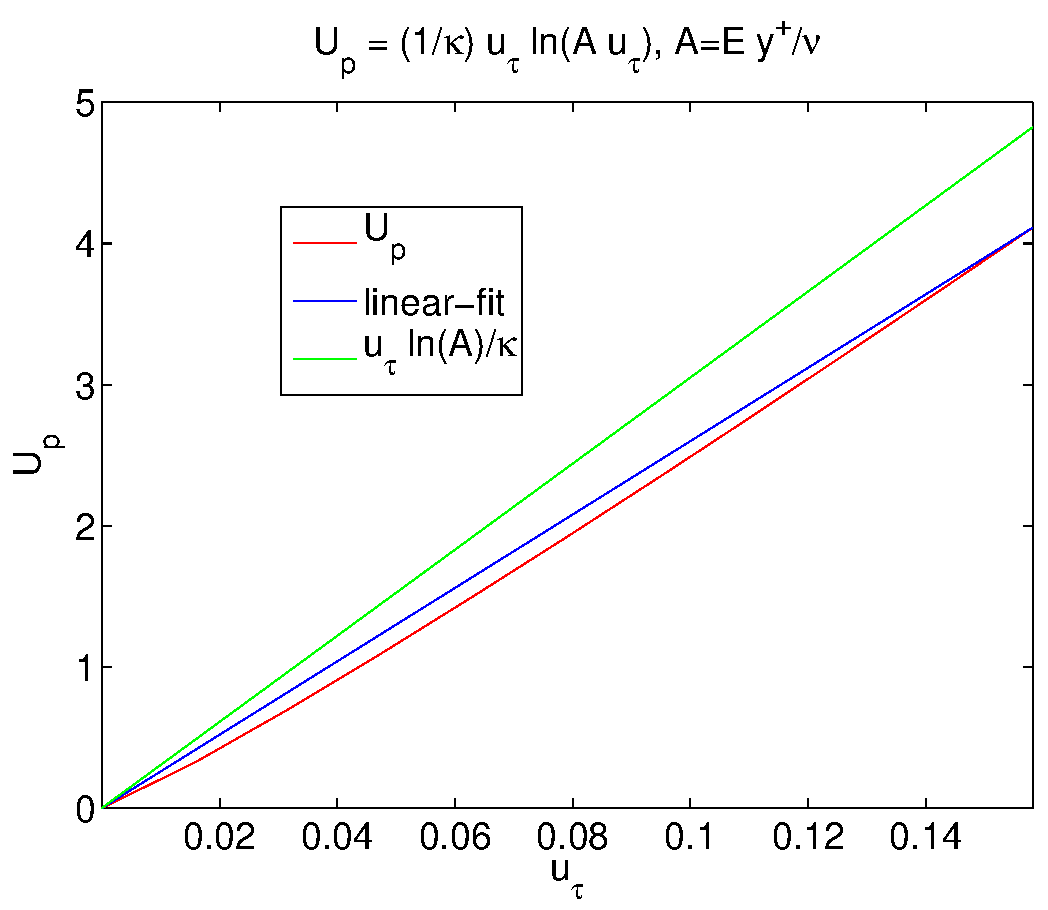
\includegraphics[width=10.cm]{\cgDoc/ins/turbulenceModels/lawOfTheWallFunction}
\end{center}
\caption{A plot of $U_p$ versus $\uTau$ for the law-of-the wall function,
             $U_p = \kappa^{-1}\uTau \ln(A \uTau)$ .}
\label{fig:lawOfTheWallFunction}
\end{figure}

%  Thus we can treat $A$ as a large parameter compared to $\tau_w$ in the expression for $G(\tau_w)$. 
%  Letting $\epsilon = 1/\ln(A)$ we can perform a perturbation expansion on $G(z)$ giving (*check this*)
%  \begin{align*}
%     z \ln( A) & = \kappa U_p - z \ln(z)  \\
%  %         \approx \kappa^{-1} z \ln( A)- U_p \\
%  \Rightarrow   z &\sim \epsilon \kappa U_p  - \kappa U_p \epsilon^2 \ln(\epsilon \kappa U_p) +O( ??)
%  \end{align*}

% 
% Let 
% \[
%   Z = \sqrt{ \tau_w} = \sqrt{ \nu U_y(x,0) } 
% \] 
% then the law of the wall formula is 
% \begin{align} 
%   U  & = {Z \over\kappa} \ln( A Z )   \leftrightarrow Z = F(U) \label{eq:low} \\
%   A& =E y_p/\nu
% \end{align}
% Then given a solution $Z_0 = F(U_0)$, where $U_0 \approx U(x,y_p)$  
% we can expand the law of the wall formula
% \begin{align}
%   Z &= F(U_0 + \delta U ) = F(U_0) + F_U(U_0)( U-U_0) + O( (U-U_0)^2 )
% \end{align}
% Differentiating the expression~\eqref{eq:low} with respect to $U$ gives (*check this*)
% \begin{align}
%   {\partial Z \over \partial U} &= F_U = { \kappa^{-1} \over 1+ \ln( A Z) }  = {  \kappa^{-1} \over 1 + \kappa U_0 / Z_0 } 
% \end{align}
% and thus 
% the boundary condition becomes (*check this*)
% \begin{align}
%   U(x,0) & = \Big(1 - 2\kappa^{-1} F_U(U_0)\Big) U(y_p) - 2\kappa^{-1}\Big( Z_0 - F_U(U_0)~U_0 \Big)
% \end{align}
% which gives a boundary condition involving $U(x,0)$ and $U(x,y_p)$ linearized about a state $(Z_0,U_0)$ that
% satisfies the law of the wall ($U_0 \approx U(x,y_p)$).

% ---------------------------
\clearpage
\subsection{Baldwin-Lomax Zero Equation Model}\label{sec:BaldwinLomax}
\newcommand{\ymax}{y_{\rm max}}
\newcommand{\Fmax}{F_{\rm max}}

The Baldwin-Lomax zero equation model is a two layer model~\cite{Wilcox}.
The inner and outer layers are given by
\begin{align*}
  \nu_T &= \begin{cases}
  \nu_{T_i} = \rho l_{\rm mix}^2 \vert \omega \vert & \text{if $y< y_c$} \\
  \nu_{T_o} = \rho \alpha C_{cp} F_{\rm wake} F_{\rm Kleb}(y;y_{\rm max}/C_{\rm Kleb}) & \text{if $y> y_c$} \\
  \end{cases} , 
\end{align*}
where
\begin{align*}
  y_c &= \min y ~~\text{such that}~~ \nu_{T_i} = \nu_{T_o}, \\
  l_{\rm mix} &= \kappa  y \Big[ 1 - e^{-y^+/A_0^+} \Big] , \\
  F_{\rm wake} &= \min\left[y_{\rm max} F_{\rm max}; C_{wk} y_{\rm max} U_{\rm dif}^2/F_{\rm max} \right] \\
  F_{\rm Kleb}(y;\delta) &= [ 1 + 5.5 (y/\delta)^6 ] ^{-1} \qquad \mbox{(Klebanoff intermittency function)} 
\end{align*}
and where $\ymax$ and $\Fmax$ are determined from the maximum of the function
\begin{align*}
  F(y) &= y \omega \Big[ 1 - e^{-y^+/A_0^+} \Big]
\end{align*}
and $\omega$ is the magnitude of the vorticity,
\begin{align*}
  \omega^2  &= (v_x-u_y)^2 + (w_y-v_z)^2 + (u_z-w_x)^2  \\
            &= 2 \Omega_{ij}\Omega_{ij} \\
     \Omega_{ij} &= \half\Big( \partial u_i/\partial x_j - \partial u_j/\partial x_i \Big)
\end{align*}
For boundary layer flows $U_{\rm dif}$ is the maximum value of $\| \uv \|$ through the layer??
For more general flows it is
\begin{align*}
  U_{\rm dif} &= \Big( \| \uv \| \Big)_{\rm max} - \Big( \| \uv \| \Big)\Big\vert_{y=\ymax}
\end{align*}
Note comment in Wilcox that $U_{\rm dif}$ is NOT the difference between the max and min velocities
as specified in the original BL paper and at {\tt http://www.cfd-online.com/Wiki/Baldwin-Lomax\_model}

The model parameters are given by
\begin{align*}
  \kappa=.40, \quad \alpha=0.0168, & \quad A_0^+ = 26 \\
  \quad C_{cp}=1.6, \quad  C_{\rm Kleb}=0.3  & \quad C_{wk} = 1 (\text{or $.25$ from cfd-online})
\end{align*}

% -------------------------------
\subsection{Spalart-Allmaras turbulence model}

Spalart-Allmaras {\bf one equation model}
\begin{align*}
  \nu_T &= \tilde{\nu} f_{v1} \\
\partial_t \tilde{\nu} + U_j \partial_j \tilde{\nu} &= c_{b1} \tilde{S} \tilde{\nu}
   - c_{w1} f_w (\tilde{\nu}/d)^2 + {1\over\sigma}\Big[  \partial_k[ (\nu+\tilde{\nu})\partial_k\tilde{\nu}]
   + c_{b2} \partial_k \tilde{\nu}\partial_k \tilde{\nu} \Big] \\
 c_{b1}=.1355, c_{b2}=.622, & c_{v1}=7.1, \sigma=2/3 \\
 c_{w1} = { c_{b1}\over\kappa^2} + {(1+c_{b2})\over\sigma},& \quad c_{w2}=0.3,\quad c_{w3}=2,\quad \kappa=.41\\
 f_{v1} = {\chi^3 \over \chi^3 + c_{v1}^3} ,& \quad f_{v2} = 1 - {\chi\over 1+\chi f_{v1}}, 
         f_w = g \left[ {1+ c_{w3}^6 \over g^6 +c_{w3}^6 }\right]^{1/6} \\
   \chi = {\tilde{\nu}\over \nu},\quad  g=r+c_{w2}(r^6-r), &\qquad r = {\tilde{\nu}\over \tilde{S}\kappa^2 d^2} \\
 \tilde{S} = S + {\tilde{\nu}\over \kappa^2 d^2} f_{v2}, &\qquad S= \sqrt{ 2 \Omega_{ij}\Omega_{ij}}  \\
\Omega_{ij} = (1/2) ( \partial_i U_j - \partial_j U_i ) & \qquad\mbox{rotation tensor}
\end{align*}
Depends on $d$, the distance to the nearest surface.

{\bf Notes}
$f_{v2}$ can be positive or negative but is bounded from above by $1$ and below by ??
\begin{align*}
   f_{v2} & = 1 - {\chi\over 1+\chi f_{v1}} \\
          & = 1 - { 1\over \chi^{-1} + 1/[1+ (c_{v1}/\chi)^{-3}] } \\
          & \rightarrow 0 \qquad\mbox{as $\chi\rightarrow \infty$} \\
          & \rightarrow 1 \qquad\mbox{as $\chi\rightarrow 0$} \\
          & \approx  1 - { 1\over (1/7) + (1/2) } = -3/4 \qquad\mbox{when $\chi=c_{v1}$}
\end{align*}
Since $f_{v2}$ can be negative, so can $r$ and $g$.

\newcommand{\figWidth}{.475\linewidth}
\begin{figure}
\begin{center}
  % \epsfig{file=\cgDoc/ins/spalGFw.eps,width=\figWidth}
  % \epsfig{file=\cgDoc/ins/spalFv.eps,width=\figWidth}
  \includegraphics[width=8.cm]{\cgDoc/ins/fig/spalGFw}
  \includegraphics[width=8.cm]{\cgDoc/ins/fig/spalFv}
\end{center}
\caption{Behaviour of the SpalartConvergence fudge functions}
\label{fig:SPAL-functions}
\end{figure}

On a rectangular grid this is discretized as
\begin{align*}
\partial_t \tilde{\nu}_\iv + U_\iv D_{0x} U_\iv + V_\iv D_{0y} U_\iv 
             &= c_{b1} \tilde{S}_\iv \tilde{\nu}_\iv
   - c_{w1} f_w (\tilde{\nu}/d)^2  \\
    & + {1\over\sigma}  D_{+x}[ (\nu+\tilde{\nu}_{i_1-\half})D_{-x} \tilde{\nu}_{\iv} 
                + D_{+y}[ (\nu+\tilde{\nu}_{i_2-\half})D_{-y} \tilde{\nu}_{\iv}] \\
    & + c_{b2} \Big\{ (D_{0x} \tilde{\nu})^2 + (D_{0y} \tilde{\nu})^2 \Big\}
\end{align*}


On curvilinear grids we use the conservative form of the second order term
\[
\grad\cdot( a \grad \phi) = {1\over J} \Big\lbrace  
        {\partial\over\partial r_1}\left( A^{11} {\partial \phi \over\partial r_1} \right) +
        {\partial\over\partial r_2}\left( A^{22} {\partial \phi \over\partial r_2} \right) + 
        {\partial\over\partial r_1}\left( A^{12} {\partial \phi \over\partial r_2} \right) + 
        {\partial\over\partial r_2}\left( A^{21} {\partial \phi \over\partial r_1} \right) \Big\rbrace 
\]
where
\begin{align*}
  A^{11} &=  a J\left[ {\partial r_1 \over \partial x_1 }^2 + {\partial r_1 \over \partial x_2 }^2 \right] \\
  A^{22} &=a J\left[ {\partial r_2 \over \partial x_1 }^2 + {\partial r_2 \over \partial x_2 }^2\right]\\
  A^{12} &= a J\left[ {\partial r_1\over\partial x_1}{\partial r_2\over\partial x_1} 
                 + {\partial r_1\over\partial x_2}{\partial r_2\over\partial x_2 } \right]
\end{align*}
A {\bf second-order accurate} compact discretization to this expression is
\[
  \grad\cdot( a \grad \phi) \approx {1\over J} \Big\lbrace
        D_{+ r_1}\left( A^{11}_{i_1-\half}D_{- r_1}\phi \right) +
        D_{+ r_2}\left( A^{22}_{i_2-\half}D_{- r_2}\phi \right) + 
        D_{0 r_1}\left( A^{12}            D_{0 r_2}\phi \right) + 
        D_{0 r_2}\left( A^{21}            D_{0 r_1}\phi \right) \Big\rbrace 
\]
where we can define the cell average values for $A^{mn}$ by
\begin{align*}
   A^{11}_{i_1-\half} &\approx \half( A^{11}_{i_1}+A^{11}_{i_1-1} ) \\
   A^{22}_{i_2-\half} &\approx \half( A^{22}_{i_2}+A^{22}_{i_2-1} )
\end{align*}


% ****************************************************************************************************
\clearpage
\newcommand{\eps}{\epsilon}
\subsection{$k-\epsilon$ turbulence model}

Here is the $k-\epsilon$ model
\begin{align*}
   \nu_T &= C_\mu k^2/\eps \\
   \partial_t k + U_j\partial_j k & = \tau_{ij} \partial_j U_i -\eps
                    + \partial_j[ (\nu+\nu_T/\sigma_k)\partial_j k] \\
    \partial_t \eps + U_j\partial_j \eps  &= C_{\eps 1} {\eps\over k}\tau_{ij} \partial_j U_i 
           -C_{\eps 2} \eps^2/k +  \partial_j[ (\nu+\nu_T/\sigma_\eps)\partial_j \eps] \\  
   C_{\eps 1}=1.44, \quad C_{\eps 2}=1.92, &\quad C_\mu = .09, \quad \sigma_k=1, \quad \sigma_\eps=1.3
\end{align*}
The production term is $P=\tau_{ij} \partial_j U_i$
\begin{align*}
  P & =\tau_{ij} \partial_j U_i \\
    & = \nuT( \partial_j U_i + \partial_i U_j) \partial_j U_i \\
    & = {\nuT\over2} ( \partial_j U_i + \partial_i U_j)( \partial_j U_i + \partial_i U_j) \\
    & = {\nuT\over2} \Big( (2 u_x)^2 + (2 v_y)^2+ (2 w_z)^2+ 2 (u_y+v_x)^2 + 2 (u_z+w_x)^2  + 2 (v_z+w_y)^2  \Big) \\
    & = \nuT\Big( 2( u_x^2 + v_y^2+ w_z^2 )+ (u_y+v_x)^2 + (u_z+w_x)^2  + (v_z+w_y)^2  \Big)
\end{align*}


{\bf Note:} Here are some references that may be useful: {\em On the implementation of the $k-\eps$ turbulence model in incompressible
         flow solvers based on a finite element discretization} by Kuzmin and Mierka (2006),
  and {\em A note on the numerical treatment of the k-epsilon turbulence model} by Lew, Buscaglia and Carrica (200?).
The authors make some recommendations on how to solve the $k-\epsilon$ equations.
We may want to adopt some of these suggestions.

% --------------------------------------------------------------------------------------------------------

\subsubsection{Full implicit solution of the k-$\eps$ turbulence model}

  The k-$\eps$ turbulence model can be solved using a {\em full-implicit} approximation.
This form is not the most memory efficient but should be more robust. 
In the full-implicit approximation, the variables $(\uv,k,\eps)$ are solved using
a fully coupled system, with the pressure being solved as a separate solve.

The implicit time-stepping procedure is described in Section~\ref{sec:implicitMultiStepNonlinear}.
% We linearize a part of the operator $\fv(\uv)$ around the state $\uvl(\xv,t)$ and write the equation as
% \begin{align}
%   \uv_t & = L(\uv; \uvl) + \big( \fv(\uv) - L(\uv; \uvl) \big) 
% \end{align} 
For the k-$\eps$ equations the implicit operator $L(\uv, k,\eps; \uv^*, k^*,\eps^*)$ is given for the $\uv$, $k$ and $\eps$ equations
by 
\begin{align*}
  L^\uv &= (\uv^*\cdot\grad)\uv + (\uv\cdot\grad)\uv^* - \grad(\nu_T^*\grad\uv) , \\ 
  L^k &=  (\uv^*\cdot\grad)k + (\uv\cdot\grad)k^* - \grad((\nu + \nu_T^*/\sigma_k)\grad k + \eps - (2 P^{*}/k^*)k + (P^*/\eps^*)\eps,  \\
  L^\eps &= (\uv^*\cdot\grad)\eps +  (\uv\cdot\grad)\eps^* - \grad((\nu + \nu_T^*/\sigma_\eps)\grad \eps 
                 - C_{\eps 1} C_\mu S_0^* k + C_{\eps 2} (e^*/k^*)^2 k + C_{\eps 2} \frac{2\eps^*}{k^*} \eps ,
\end{align*}
where $\nu_T^* =C_\mu (k^*)^2/\eps^* $. 
% 
% 
% We first {\em linearize} the equations about a given {\em star} state $\uv^{*}$, $k^*$, $\eps^*$.
% For example:
% \begin{align*}
%    (\uv\cdot\grad)\uv &= (\uv^*\cdot\grad)\uv + (\uv\cdot\grad)\uv^*  +  ((\uv-\uv^*)\cdot\grad)\uv + (\uv\cdot\grad)(\uv-\uv^*), \\
%    \grad(\nu_T\grad\uv) &= \grad(\nu_T^*\grad\uv) + \grad((\nu_T-\nu_T^*)\grad\uv) .
% \end{align*}
% 
% The full implicit approximation solves the linearized equations using the two-level $\theta$-scheme that reduces to Backward-Euler in time
% for $\theta=0$ and Crank-Nicolson for $\theta=\half$, 
% \begin{align*}
%   {\Uv_\iv^{n+1} - \Uv_\iv^n \over \dt} & + (1-\theta)\Big[ (\Uv_\iv^*\cdot\grad_h)\Uv_\iv^{n+1} + 
%                  (\Uv_\iv^{n+1}\cdot\grad_h)\Uv_\iv^{*} 
%      - \grad_h( (\nu+\nu_T^{*} \grad \Uv_\iv^{n+1} ) \Big] = \Rv_\uv^n \\
%  {k_\iv^{n+1} - k_\iv^n \over \dt} & + (1-\theta)\Big[ (\Uv_\iv^*\cdot\grad_h)k_\iv^{n+1} + (\Uv_\iv^{n+1}\cdot\grad_h)k_\iv^{*} 
%          - \grad_h( (\nu+\nu_T^{*}/\sigma_k \grad k_\iv^{n+1} ) ) \\
%      &    +  \eps^{n+1}  - (2 P^{*}/k^*)k^{n+1} + (P^*/\eps^*)\eps^{n+1} \Big]
%      = R_k^n
% \end{align*}
% where the right-hand sides are given by 
% \begin{align*}
%   \Rv_\uv^n &= \theta\Big[ 
%            -  (\Uv_\iv^*\cdot\grad_h)\Uv_\iv^{n} -  (\Uv_\iv^n\cdot\grad_h)\Uv_\iv^{*} 
%            + \grad_h( (\nu+\nu_T^{*} \grad \Uv_\iv^{n} ) )   \Big] \\
%           & -  \grad_h p_\iv^n  + (\Uv_\iv^*\cdot\grad_h)\Uv_\iv^{*} + \grad_h( (\nu_T-\nu_T^{*}) \grad \Uv_\iv^{n} )      \\
%   R_k^n &= \theta\Big[ -(\Uv_\iv^n\cdot\grad_h)k_\iv^{n} +  P(\Uv_\iv^n)  + \grad_h( (\nu+\nu_T^{n}/\sigma_k \grad k_\iv^{n} ) ) \Big] 
% \end{align*}
Here the {\em star} states $\uv^{*}$, $k^*$, and $\eps^*$ denote the states that are used to linearize the equations. 
A large sparse matrix is formed for the implicit system and this is kept fixed for some number of
time steps (chosen by the {\tt refactor frequency} option).


Notes:
\begin{enumerate}
  \item The main implicit time-stepping routine is in {\tt common/src/ims.C}. 
      The RHS for the implicit solve is computed ins {\tt ins/src/ins.C}. 
  \item The file {\tt ins/src/insImpKE.bf} defines the implicit system that is solved for the k-$\eps$ equations.
  \item The file {\tt ins/src/insImp.h} defines some generic macros and subroutines that are used for different
    implicit solvers (including the k-$\eps$ and Baldwin-Lomax equations, {\tt insImpBL.bf}).
  \item The file {\tt ins/src/turbulenceModels.C} defines the boundary conditions for the turbulence models
      used for explicit time stepping and currently these are also used for the implicit time steppers.
  \item The fortran routines are called from the C++ file {\tt ins/src/implicit.C} in function {\tt insImplicitMatrix}.
\end{enumerate}


% ****************************************************************************************************
\subsection{Diffusion Operator}

When a turbulence model is added to the incompressible Navier-Stokes equation the diffusion
operator usually takes the form of 
\begin{align*}
   {\cal D}_i &= \sum_j \partial_{x_j} \Big( \nuT (\partial_{x_i} u_j + \partial_{x_j} u_i) \Big) 
\end{align*}
where we will write  $\nuT$ instead of $\nu+\nuT$ in this section.
In particular
\begin{align*}
   \Dopu &= \partial_x( 2\nuT u_x) + \partial_y( \nuT u_y) + \partial_z( \nu_T u_z ) 
                    + \partial_y( \nuT v_x ) + \partial_z( \nu_T w_x ) \\
   \Dopv &= \partial_x( \nuT v_x) + \partial_y(2\nuT v_y) + \partial_z( \nu_T v_z ) 
                    + \partial_x( \nuT u_y ) + \partial_z( \nu_T w_y ) \\
   \Dopw &= \partial_x( \nuT w_x) + \partial_y( \nuT w_y) + \partial_z(2\nu_T w_z ) 
                    + \partial_y( \nuT v_z ) + \partial_x( \nu_T u_z ) \\
\end{align*}
We can write these in a more ``symmetric'' form as follows.
Since $u_x+v_y+w_z=0$, it follows that 
\[
   \partial_x( \nuT u_x) = -\partial_x( \nuT v_y ) -\partial_x( \nuT w_z ) 
\]
and thus 
\begin{align*}
 \Dopu &= \partial_x ( \nuT u_x) + \partial_y( \nuT u_y) + \partial_z( \nu_T u_z ) 
               + \partial_y( \nuT v_x ) -\partial_x( \nuT v_y ) + \partial_z( \nu_T w_x )-\partial_x( \nuT w_z )
\end{align*}
Therefore the diffusion operator can be written in a form where the principle part is the 
same for all components,
\begin{align*}
 \Dopu &= \grad\cdot( \nuT \grad u) + \partial_y( \nuT v_x ) -\partial_x( \nuT v_y ) 
                                         + \partial_z( \nuT w_x ) -\partial_x( \nuT w_z ) \\
 \Dopv &= \grad\cdot( \nuT \grad v) + \partial_z( \nuT w_y ) -\partial_y( \nuT w_z ) 
                                         + \partial_x( \nuT u_y ) -\partial_y( \nuT u_x ) \\
 \Dopw &= \grad\cdot( \nuT \grad w) + \partial_x( \nuT u_z ) -\partial_z( \nuT u_x ) 
                                         + \partial_y( \nuT v_z ) -\partial_z( \nuT v_y ) 
\end{align*}
Note that the highest order derivatives cancel in the last four terms in these expressions,\begin{align*}
 \Dopu &= \grad\cdot( \nuT \grad u) + \partial_y( \nuT) v_x -\partial_x(\nuT) v_y  
                                         + \partial_z( \nuT) w_x -\partial_x(\nuT) w_z  \\
 \Dopv &= \grad\cdot( \nuT \grad v) + \partial_z( \nuT) w_y -\partial_y(\nuT) w_z  
                                         + \partial_x( \nuT) u_y -\partial_y(\nuT) u_x  \\
 \Dopw &= \grad\cdot( \nuT \grad w) + \partial_x( \nuT) u_z -\partial_z(\nuT) u_x  
                                         + \partial_y( \nuT) v_z -\partial_z(\nuT) v_y  
\end{align*}

\subsection{Revised pressure equation}


When a turbulence model is added to the incompressible Navier-Stokes equation the diffusion
operator usually takes the form of 
\begin{align*}
   {\cal D}_i &= \sum_j \partial_{x_j} \Big( \nuT (\partial_{x_i} u_j + \partial_{x_j} u_i) \Big) 
\end{align*}


The pressure equation is derived from taking the divergence of the momentum equations,
\[
   \partial_t \uv + (\uv\cdot\grad)\uv + \grad p = {\bf\cal D}
\]
and using $\grad\cdot\uv=0$ to give
\[
    \Delta p = - \grad\uv:\grad\uv  + \grad\cdot{\bf\cal D}
\]
For a constant viscosity, the last term on the right hand side is zero.
When the viscosity is not constant we need to include the divergence of the 
diffusion operator in the equation for the pressure. This takes the form
\begin{align*}
   \grad\cdot{\cal D} &= 
           \sum_i\sum_j \partial_{x_i}\partial_{x_j}\Big[ 
                     \nuT\Big( \partial_{x_j} u_i + \partial_{x_i} u_j \Big)
                                   \Big] \\
         &= \sum_j\partial_{x_j}\Big[ \sum_i\partial_{x_i}\nuT~\partial_{x_j} u_i \Big]
           +\sum_i\partial_{x_i}\Big[ \sum_j\partial_{x_j}\nuT~\partial_{x_i} u_j \Big] \\
         &= 2~\sum_i\partial_{x_i}\Big[ \sum_j~\partial_{x_j}\nuT~\partial_{x_i} u_j \Big]
\end{align*}
where we have again used $\grad\cdot\uv=0$.

In two dimensions this takes the form
\begin{align*}
   \grad\cdot{\cal D}^{\rm(2d)}
         &= 2~\Big[ \partial_x\Big( \partial_x\nuT~\partial_x u + \partial_y\nuT~\partial_x v \Big)+
                    \partial_y\Big( \partial_x\nuT~\partial_y u + \partial_y\nuT~\partial_y v \Big)
              \Big] \\
         &=2~\Big[ \partial_x\nuT~\Delta u + \partial_x^2\nuT~\partial_x u +\partial_x\partial_y\nuT~\partial_y u \\
         &~~~~~    + \partial_y\nuT~\Delta v + \partial_x\partial_y\nuT~\partial_x v+ \partial_y^2\nuT~\partial_y v
              \Big]
\end{align*}
In three dimensions,
\begin{align*}
   \grad\cdot{\cal D}^{\rm(3d)}
 &= 2~\Big[
   \partial_x\Big( \partial_x\nuT~\partial_x u+\partial_y\nuT~\partial_x v+\partial_z\nuT~\partial_x w \Big) \\
&~~~~~  +\partial_y\Big( \partial_x\nuT~\partial_y u+\partial_y\nuT~\partial_y v+\partial_z\nuT~\partial_y w \Big) \\
&~~~~~  +\partial_z\Big( \partial_x\nuT~\partial_z u+\partial_y\nuT~\partial_z v+\partial_z\nuT~\partial_z w \Big)
              \Big] \\
   &=2~\Big[ \partial_x\nuT~\Delta u + \partial_x^2\nuT~\partial_x u +\partial_x\partial_y\nuT~\partial_y u
                            +\partial_x\partial_z\nuT~\partial_z u        \\
   &~~~~~    + \partial_y\nuT~\Delta v + \partial_x\partial_y\nuT~\partial_x v+ \partial_y^2\nuT~\partial_y v
                           + \partial_y\partial_z\nuT~\partial_z v \\
   &~~~~~    + \partial_z\nuT~\Delta w + \partial_x\partial_z\nuT~\partial_x w
                           + \partial_y\partial_z\nuT~\partial_y w
                           + \partial_z^2\nuT~\partial_z w 
              \Big]
\end{align*}

\newcommand{\sgn}[1]{{\rm sgn}(#1)}

The addition of artificial dissipation also changes the pressure equation.
The second-order artificial dissipation is 
\begin{equation} 
   \dv_{2,i} =
    \left( {\ff ad21} + {\ff ad22} | \grad_h \Vv_i |_1
    \right) \sum_{m=1}^{n_d} \Delta_{m+}\Delta_{m-} \Vv_i
\end{equation}
while the the fourth-order one is
\begin{equation} 
   \dv_{4,i} =
  - \left( {\ff ad41} + {\ff ad42} | \grad_h \Vv_i |_1
    \right) \sum_{m=1}^{n_d} \Delta_{m+}^2\Delta_{m-}^2 \Vv_i
\end{equation}

The artificial dissipation is of the form 
\begin{align*}
 \dv &=  \Big[ \alpha_0 + \alpha_1 {\cal G}(\grad\uv) \Big] \sum_{m=1}^{n_d} \Delta_{m+}^p\Delta_{m-}^p \uv \\
   {\cal G}(\grad\uv) &= |u_x| + |u_y| + |v_x| + |v_y| + \ldots
\end{align*}
Taking the divergence of this expression results in
\begin{align*}
\grad\cdot\dv &=  \alpha_1\Big[ {\cal G}_x \sum_{m}\Delta_{m+}^p\Delta_{m-}^p U 
                              + {\cal G}_y \sum_{m}\Delta_{m+}^p\Delta_{m-}^p V \Big]
\end{align*}
where
\begin{align*}
  {\cal G}_x &= \sgn{u_x}~u_{xx} + \sgn{u_y}~u_{xy}+ \sgn{v_x}~v_{xx}+ \sgn{v_y}~v_{xy}+\ldots
\end{align*}
and $\sgn{x}$ is $+1$, $-1$ or $0$ for $x>0$, $x<0$ or $x=0$.


\subsubsection{Revised pressure boundary condition}

The {\em pressure boundary condition} also is changed to include the new
diffusion operator:
\[
  \partial_n p = \nv\cdot\Big\{ -\partial_t \uv -(\uv\cdot\grad)\uv + {\cal D} \Big\}
\]
We would like to write the diffusion operator in a way similiar to {\em curl-curl}  form, 
\[
\Delta\uv=-\grad\times\grad\times \uv+\grad(\grad\cdot\uv), 
\]
used in the INS equations. Expanding the expression for $\Dopu$ gives
\begin{align*}
   \Dopu &= \partial_x( 2\nuT u_x) + \partial_y( \nuT u_y) + \partial_z( \nu_T u_z ) 
                    + \partial_y( \nuT v_x ) + \partial_z( \nu_T w_x ) \\
              &= 2\nuT u_{xx} + \nuT u_{yy} + \nuT u_{zz} + 2\partial_x \nuT u_x 
                    + \partial_y\nuT( u_y+v_x)  + \partial_z\nuT( u_z + w_x )
                     + \nuT( v_{xy} + w_{xz} ) \\
              &= \nuT \Delta u + 2\partial_x \nuT u_x + \partial_y\nuT( u_y+v_x) + \partial_z\nuT( u_z + w_x )
\end{align*}
where we have used $v_{xy} + w_{xz} = - u_{xx}$
Thus we can write
\begin{align*}
   \Dopu &=  \nuT \Delta u - 2\partial_x \nuT (v_y+w_z) + \partial_y\nuT( u_y+v_x) + \partial_z\nuT( u_z + w_x )
\end{align*}
This leads in two dimensions to the {\em curl-curl} form
\begin{align}
   \Dopu^{(2D)} &= \nuT(-v_{xy}+u_{yy}) - 2\partial_x \nuT v_y + \partial_y\nuT( u_y+v_x ) \label{eq:curl2d-u} \\
   \Dopv^{(2D)} &= \nuT(~~v_{xx}-u_{xy})- 2\partial_y \nuT u_x + \partial_x\nuT( v_x+u_y ) \label{eq:curl2d-v}
\end{align}
while in three dimensions,
\begin{align}
   \Dopu &=  \nuT(-v_{xy}-w_{xz}+u_{yy}+u_{zz}) - 2\partial_x \nuT (v_y+w_z)
                       + \partial_y\nuT( u_y+v_x) + \partial_z\nuT( u_z + w_x )  \label{eq:curl3d-u} \\
   \Dopv &=  \nuT(~~v_{xx}-u_{xy}-w_{yz}+v_{zz}) - 2\partial_y \nuT (w_z+u_x) 
                       + \partial_z\nuT( v_z+w_y) + \partial_x\nuT( v_x + u_y )  \label{eq:curl3d-v} \\
   \Dopw &=  \nuT(~~w_{xx}+w_{yy}-u_{xz}-v_{yz}) - 2\partial_z \nuT (u_x+v_y) 
                       + \partial_x\nuT( w_x+u_z) + \partial_y\nuT( w_y + v_z ) \label{eq:curl3d-w} 
\end{align}   
These {\em curl-curl} forms~(\ref{eq:curl2d-u}-\ref{eq:curl3d-w}) remove the normal derivatives of the
normal components of the velocity from $\nv\cdot(\Dopu,\Dopv,\Dopw)$. 
For example, the expression for $\Dopu$ contains no $x$-derivatives of $u$
while $\Dopv$ contains no $y$-derivatives of v.

The alternative conservative form is 
\begin{align*}
   \Dopu &= \partial_x( -2\nuT(v_y+w_z)) + \partial_y( \nuT u_y) + \partial_z( \nu_T u_z ) 
                    + \partial_y( \nuT v_x ) + \partial_z( \nu_T w_x ) \\
   \Dopv &= \partial_x( \nuT v_x) + \partial_y(-2\nuT(u_x+w_z)) + \partial_z( \nu_T v_z ) 
                    + \partial_x( \nuT u_y ) + \partial_z( \nu_T w_y ) \\
   \Dopw &= \partial_x( \nuT w_x) + \partial_y( \nuT w_y) + \partial_z(-2\nu_T(u_x+v_y) ) 
                    + \partial_y( \nuT v_z ) + \partial_x( \nu_T u_z ) \\
\end{align*}





